\section{Auswertung}
\label{sec:Auswertung}
\subsection{Stehende Schallwellen}
\label{subsec:Stehende Schallwellen}
Abbildung \ref{fig:1-1} zeigt das Übersichtsspektrum der 600~mm Röhre von 0.1~kHz bis 10~kHz.
\begin{figure}
\centering
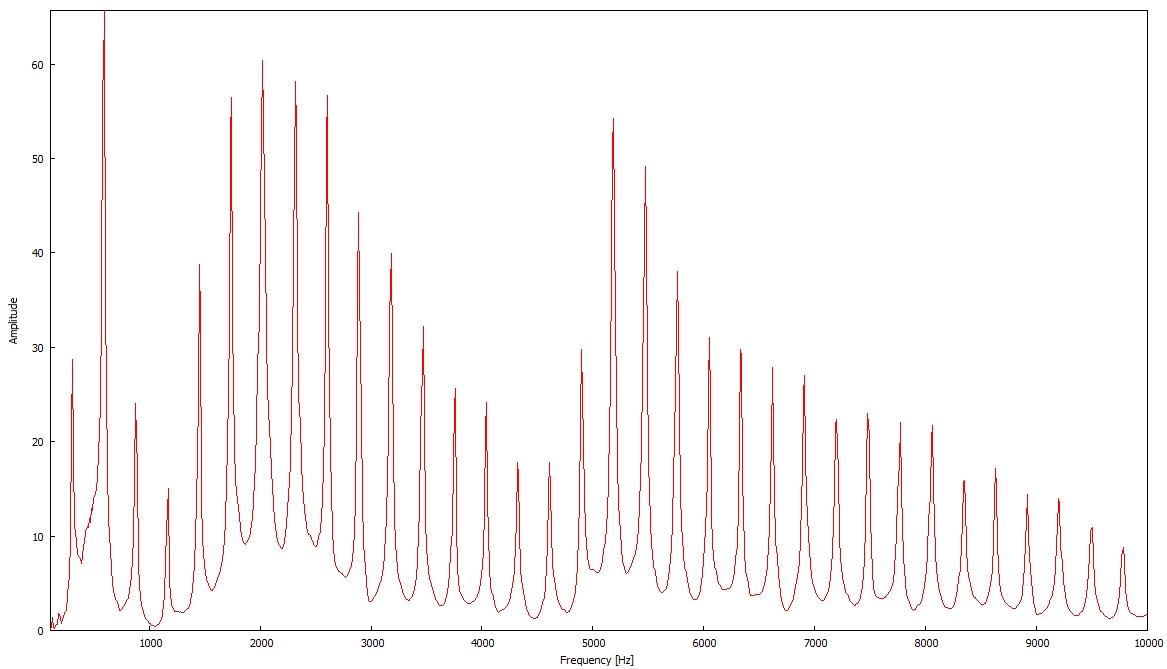
\includegraphics[width=\textwidth]{content/messungen/Chapter1/1-1img.jpg}
\caption{Übersichtsspektrum der Schallwellen in einer 600~mm langen Röhre von 0.1~kHz bis 10~kHz.}
\label{fig:1-1}
\end{figure}

Die zwei von 5~kHz bis 14~kHz aufgenommenen Spektren der 150~mm Röhre sind in den Abbildungen \ref{fig:1-2a:a} und \ref{fig:1-2b:a} dargestellt.
Zu diesen beiden Spektren sind die entsprechenden Fits in den Abbildungen \ref{fig:1-2a:b} und \ref{fig:1-2b:b} dargestellt.
Die vom Messprogramm ,,SpektrumSLC.exe'' erstellten Parameter, die die Peaks des Spektrums charakterisieren, sind in Tabelle \ref{tab:1:1} bzw. in Tabelle \ref{tab:1:2} aufgeführt.
%%%%%%%%%%%%%%%%%%%%%%%%%%
\begin{figure}
\centering
\begin{subfigure}{0.4\textwidth}
\vspace{0.8cm}
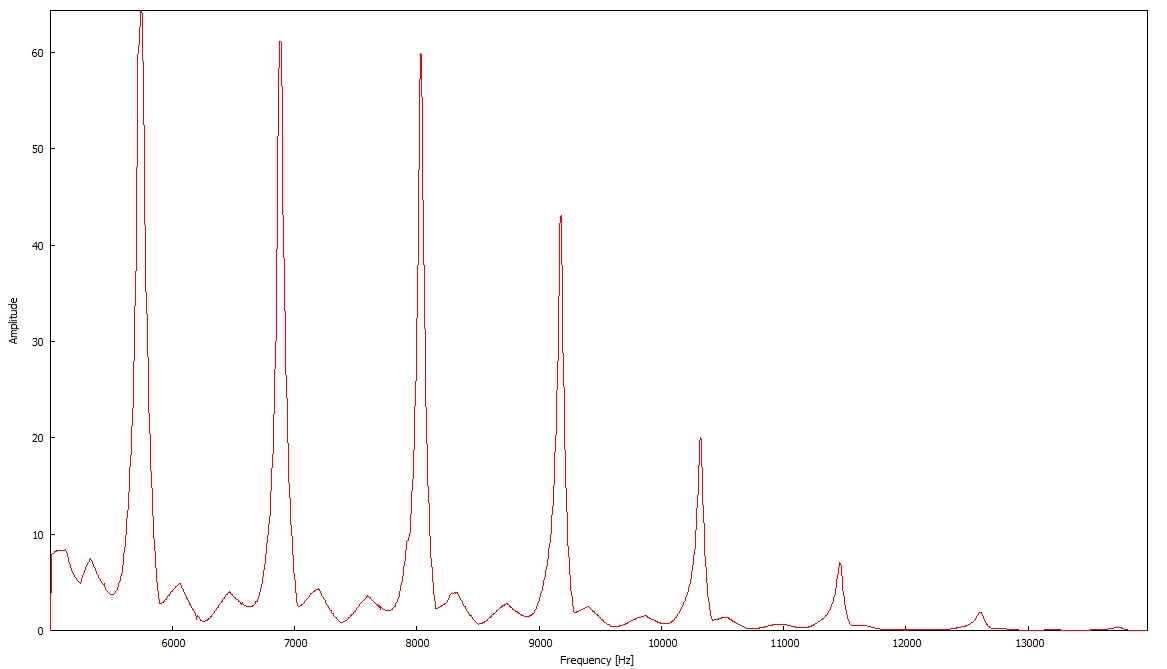
\includegraphics[width=\textwidth]{content/messungen/Chapter1/1-2img.jpg}
\subcaption{Rohdaten}
\label{fig:1-2a:a}
\end{subfigure}
\begin{subfigure}{0.4\textwidth}
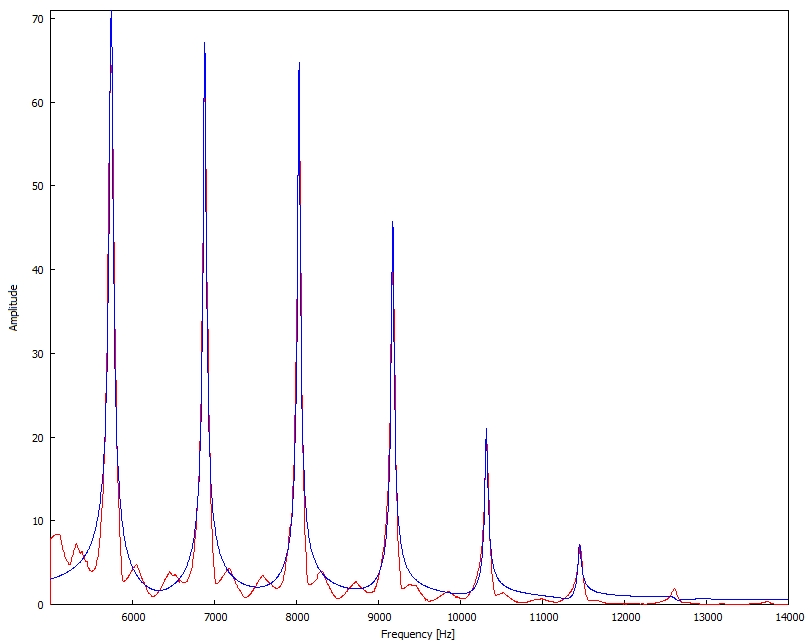
\includegraphics[width=\textwidth]{content/messungen/Chapter1/fit_img1.jpg}
\subcaption{Rohdaten mit Fit. Für Fitparameter siehe Tabelle \ref{tab:1:1}}
\label{fig:1-2a:b}
\end{subfigure}
\caption{Spektrum einer 150~mm langen Rühre von 5~kHz bis 14~kHz.}
\label{fig:1-2a}
\end{figure}
%%%%%%%%%%%%%%%%%%%%%%%%%%

%%%%%%%%%%%%%%%%%%%%%%%%%%
\begin{figure}
\centering
\begin{subfigure}{0.4\textwidth}
\vspace{0.8cm}
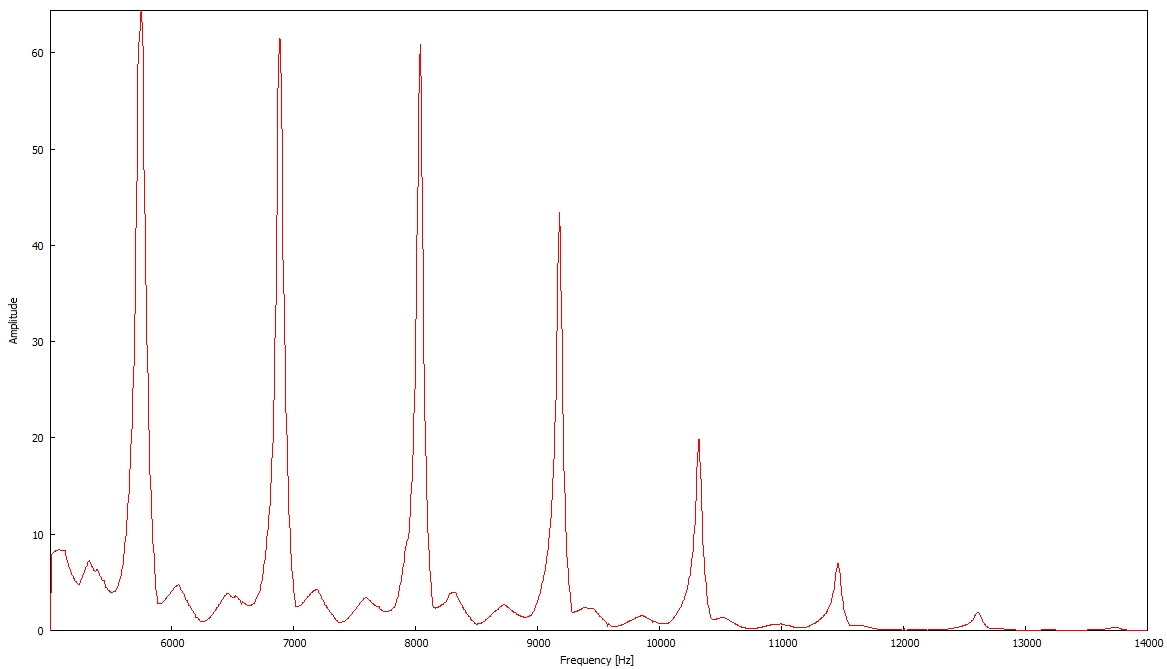
\includegraphics[width=\textwidth]{content/messungen/Chapter1/1-2-2img.jpg}
\subcaption{Rohdaten}
\label{fig:1-2b:a}
\end{subfigure}
\begin{subfigure}{0.4\textwidth}
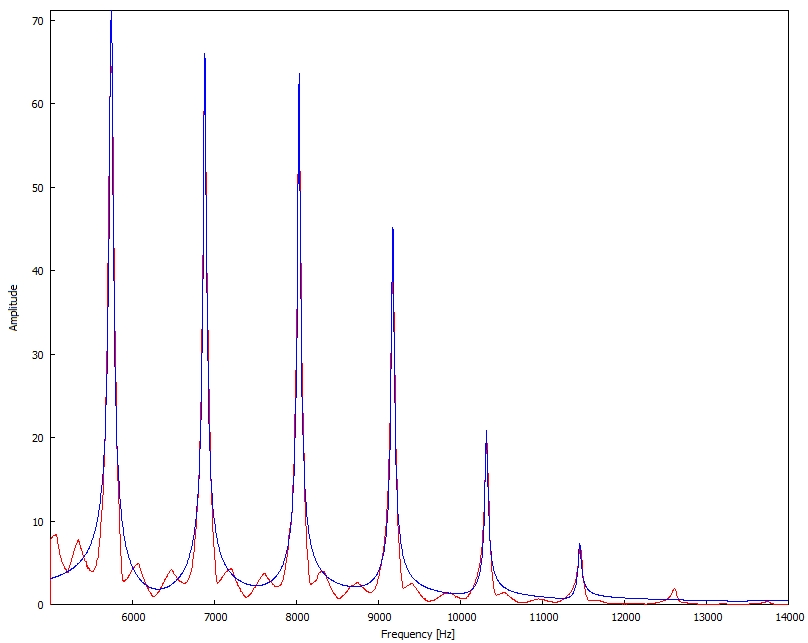
\includegraphics[width=\textwidth]{content/messungen/Chapter1/fit_img2.jpg}
\subcaption{Rohdaten mit Fit. Für Fitparameter siehe Tabelle \ref{tab:1:1}}
\label{fig:1-2b:b}
\end{subfigure}
\caption{Wiederholungsmessung des Spektrums einer 150~mm langen Rühre von 5~kHz bis 14~kHz.}
\label{fig:1-2b}
\end{figure}
%%%%%%%%%%%%%%%%%%%%%%%%%%

\begin{table}
\centering
\caption{Ergebnis des Fits aus Abbildung \ref{fig:1-2a}.}
\label{tab:1:1}
\begin{tabular}{c c c c c c c c c}
\hline
 & Peak 1 & Peak 2 & Peak 3 & Peak 4 & Peak 5 & Peak 6&Peak 7&Peak 8 \\ \hline

Frequenz in Hz& 5750&6890&8030&9180&10300&11500&12600&17200\\
Amplitude&69.9&65.8&63.5&44.6&20.0&6.45&0.41&0.20\\
Breite in Hz&21.3&16.6&14.6&15.0&16.2&20.1&52.1&4200\\
Phase in Grad&-51.0&-31.2&4.3&38.2&57.5&50.5&-140&178\\
\hline
\end{tabular}
\end{table}

\begin{table}
\centering
\caption{Ergebnis des Fits aus Abbildung \ref{fig:1-2b}.}
\label{tab:1:2}
\begin{tabular}{c c c c c c c c c}
\hline
 & Peak 1 & Peak 2 & Peak 3 & Peak 4 & Peak 5 & Peak 6&Peak 7&Peak 8 \\ \hline

Frequenz in Hz&5750&6890&8030&9180&10300&11500&13500&13700\\
Amplitude&70.0&64.8&62.0&44.1&19.9&6.60&0.02&0.18\\
Breite in Hz&21.3&17.5&15.8&15.6&16.2&18.2&512&230\\
Phase in Grad&-46.5&-26.1&9.90&51.2&72.3&72.5&-107&37.0\\
\hline
\end{tabular}
\end{table}
\FloatBarrier
\subsection{Der Kugelresonator}
\label{subsec:Der Kugelresonator}
Die Übersichtsspektren für die Winkel $\alpha=0\degree,30\degree,60\degree,90\degree,120\degree,150\degree,180\degree$ werden in den Abbildung \ref{fig:2_1_0} bis \ref{fig:2_1_180} dargestellt.
%%%%%%%%%%%%%%%%%%%%%%%%
\begin{figure}
\centering
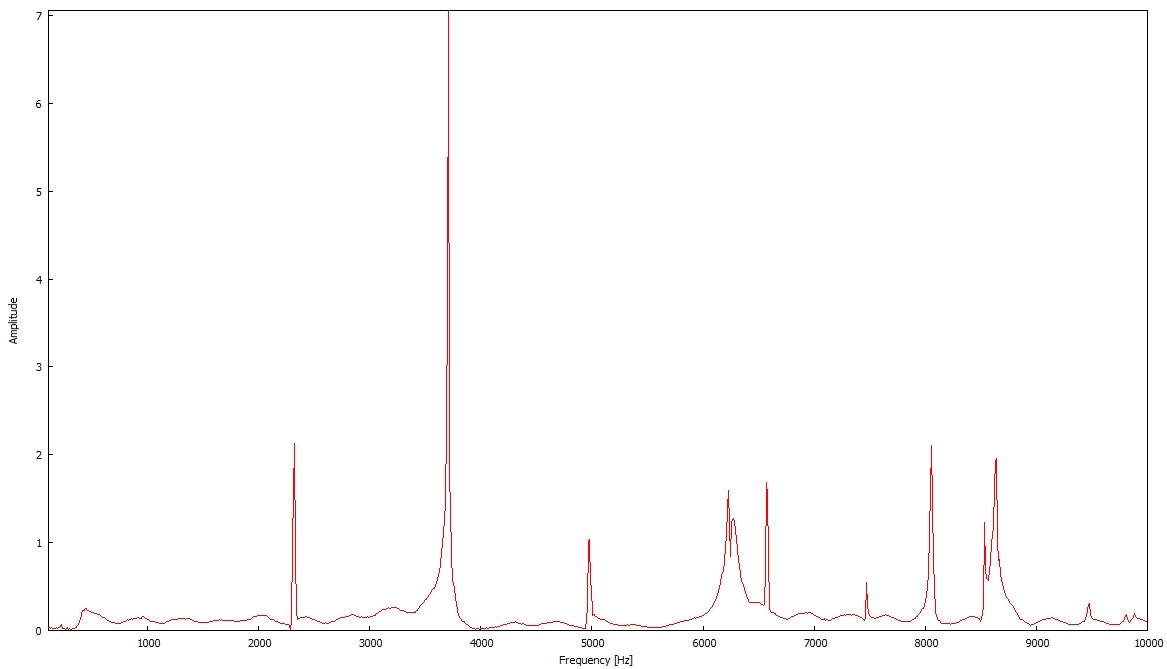
\includegraphics[width=\textwidth]{content/messungen/Chapter2new/2_1_0img.jpg}
\caption{Übersichtsspektrum des Kugelresonators von 0.1~kHz bis 10~kHz für $\alpha=0\degree$.}
\label{fig:2_1_0}
\end{figure}

\begin{figure}
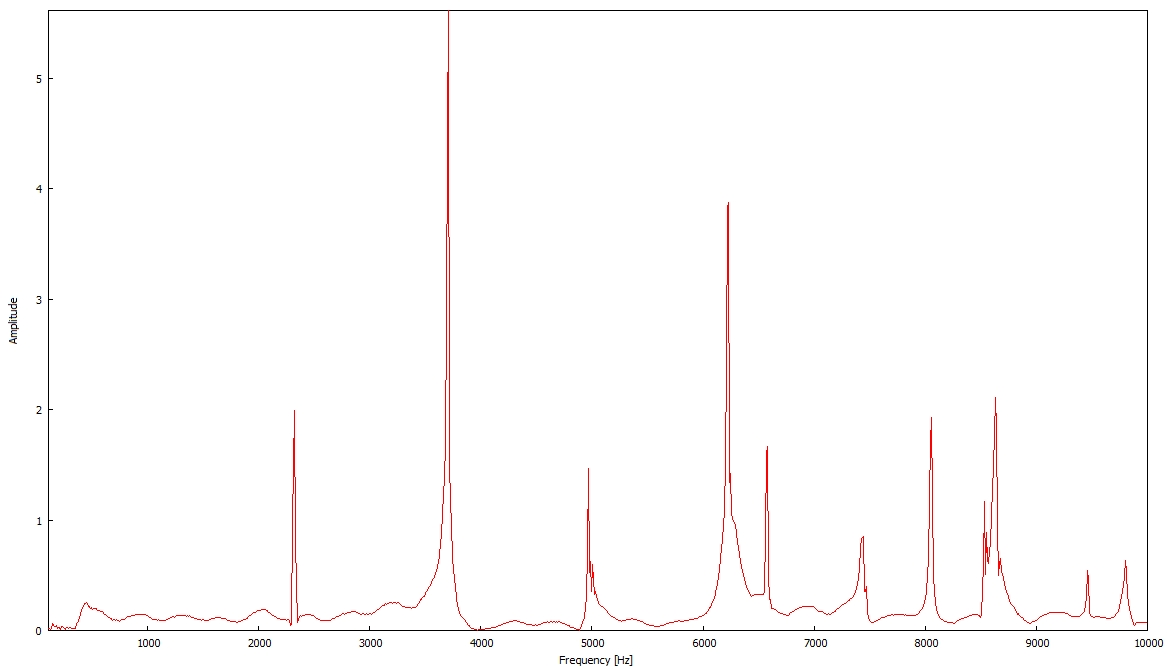
\includegraphics[width=\textwidth]{content/messungen/Chapter2new/2_1_30img.jpg}
\caption{Übersichtsspektrum des Kugelresonators von 0.1~kHz bis 10~kHz für $\alpha=30\degree$.}
\label{fig:2_1_30}
\end{figure}

\begin{figure}
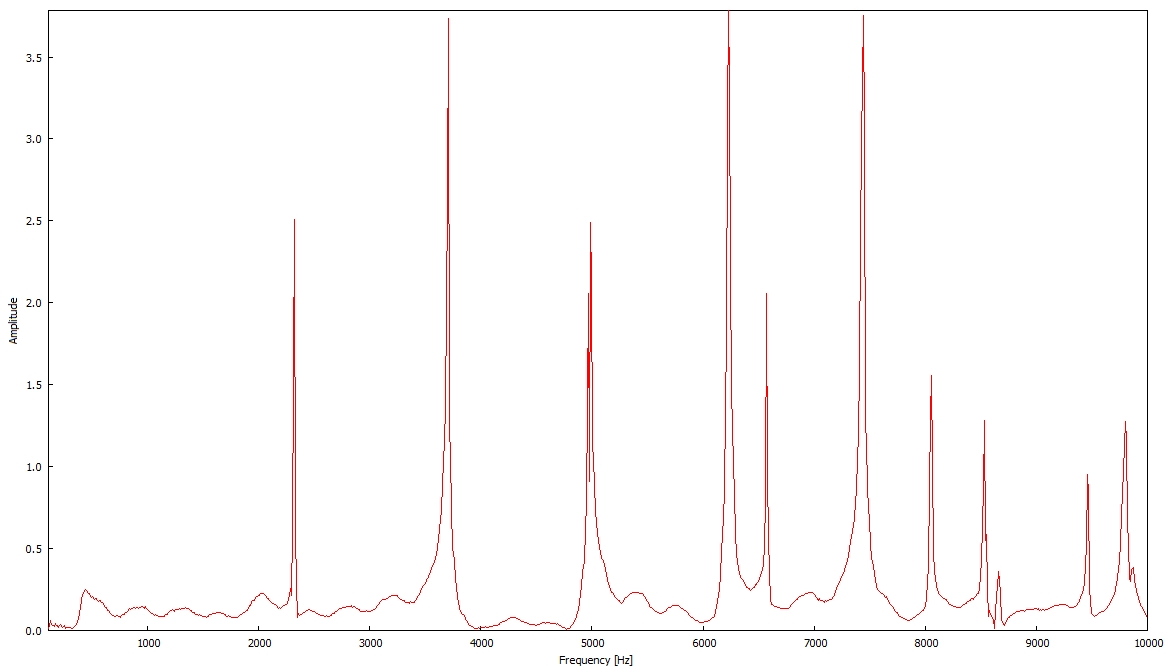
\includegraphics[width=\textwidth]{content/messungen/Chapter2new/2_1_60img.jpg}
\caption{Übersichtsspektrum des Kugelresonators von 0.1~kHz bis 10~kHz für $\alpha=60\degree$.}
\label{fig:2_1_60}
\end{figure}

\begin{figure}
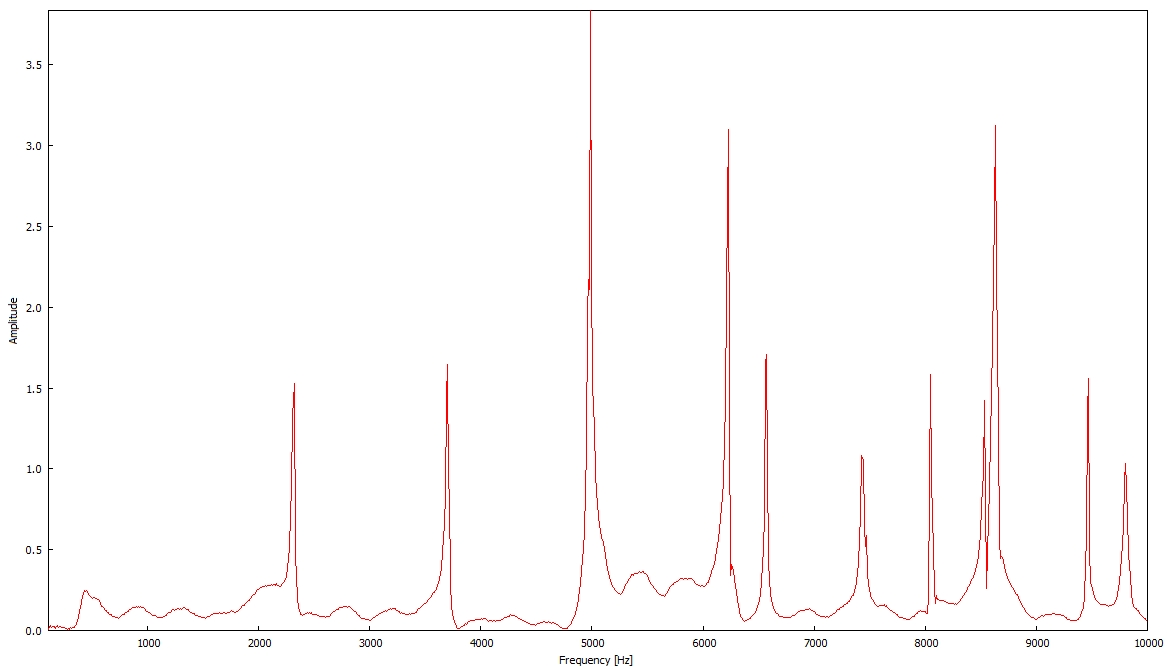
\includegraphics[width=\textwidth]{content/messungen/Chapter2new/2_1_90img.jpg}
\caption{Übersichtsspektrum des Kugelresonators von 0.1~kHz bis 10~kHz für $\alpha=90\degree$.}
\label{fig:2_1_90}
\end{figure}

\begin{figure}
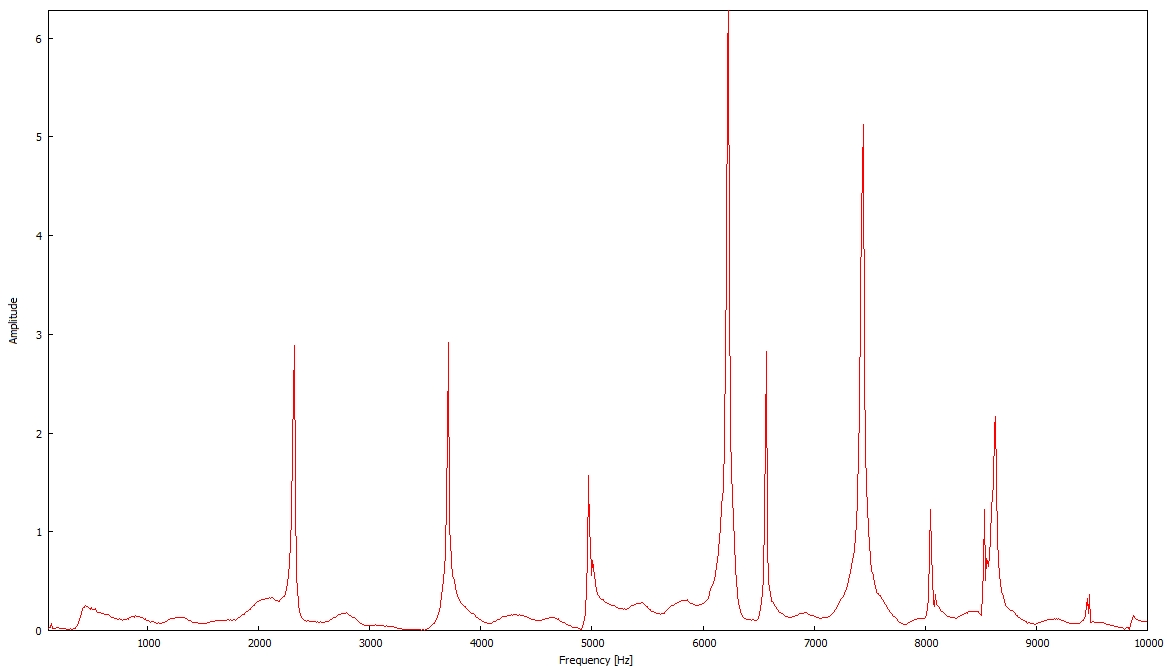
\includegraphics[width=\textwidth]{content/messungen/Chapter2new/2_1_120img.jpg}
\caption{Übersichtsspektrum des Kugelresonators von 0.1~kHz bis 10~kHz für $\alpha=120\degree$.}
\label{fig:2_1_120}
\end{figure}

\begin{figure}
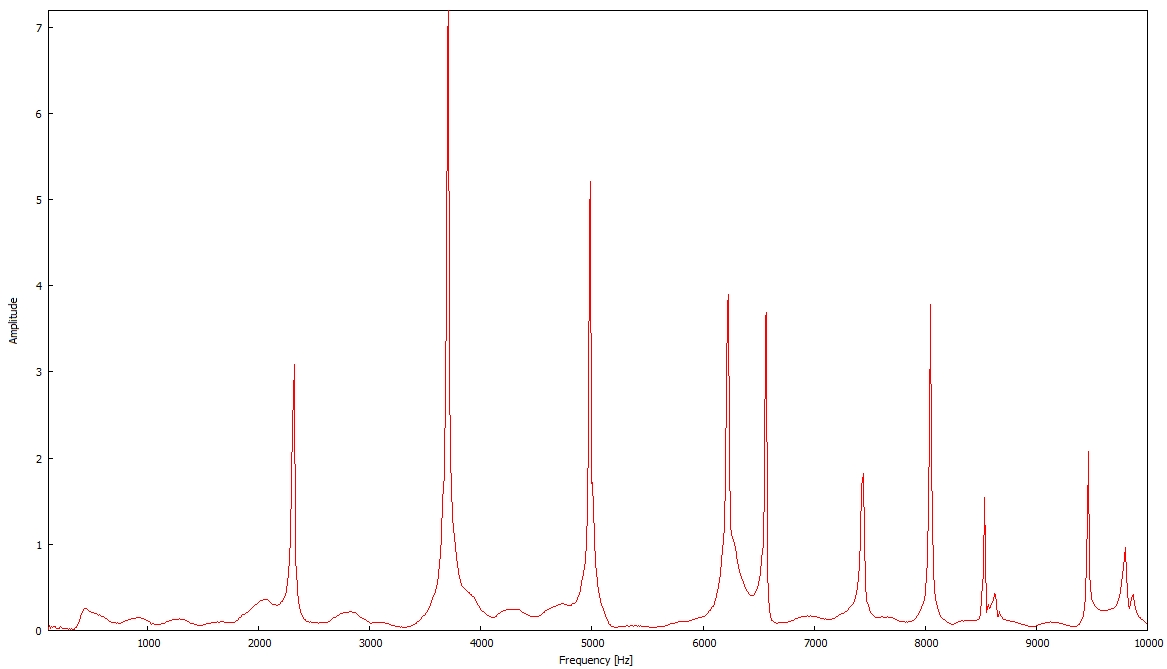
\includegraphics[width=\textwidth]{content/messungen/Chapter2new/2_1_150img.jpg}
\caption{Übersichtsspektrum des Kugelresonators von 0.1~kHz bis 10~kHz für $\alpha=150\degree$.}
\label{fig:2_1_150}
\end{figure}

\begin{figure}
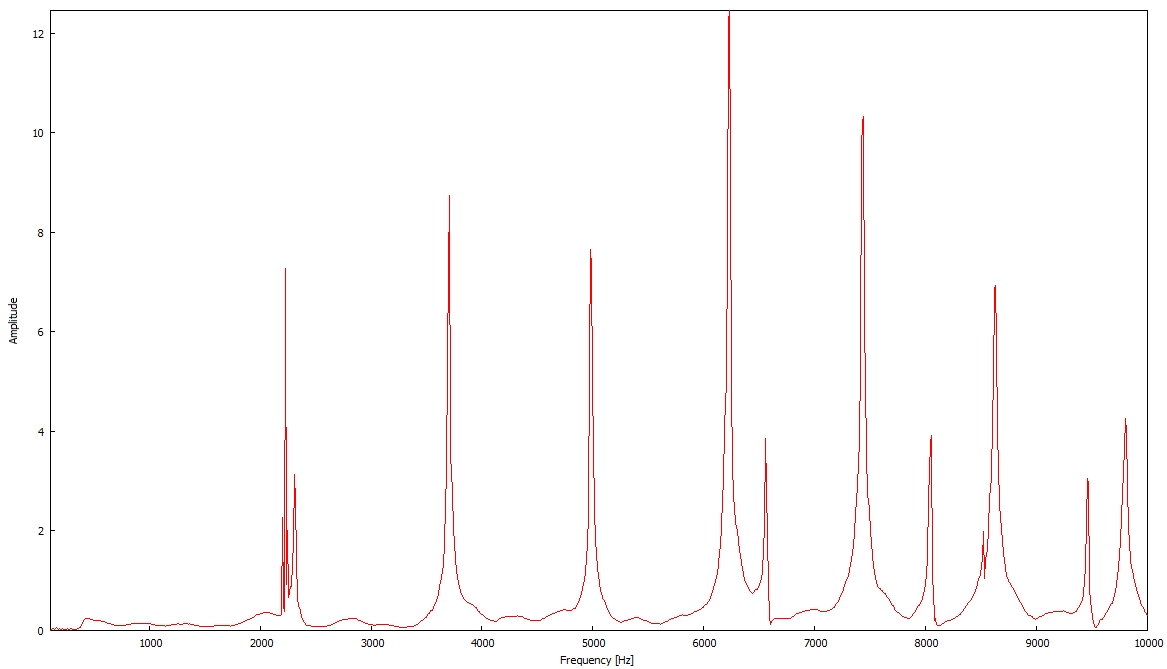
\includegraphics[width=\textwidth]{content/messungen/Chapter2new/2_1_180img.jpg}
\caption{Übersichtsspektrum des Kugelresonators von 0.1~kHz bis 10~kHz für $\alpha=180\degree$.}
\label{fig:2_1_180}
\end{figure}
%%%%%%%%%%%%%%%%%%%%%%%%%%%%%
Die Abbildungen \ref{fig:2_2_0} bis \ref{fig:2_2_40} zeigen die Untersuchungsergebnisse der Resonanzstelle bei ca. 5~kHz. 
\begin{figure}
\centering
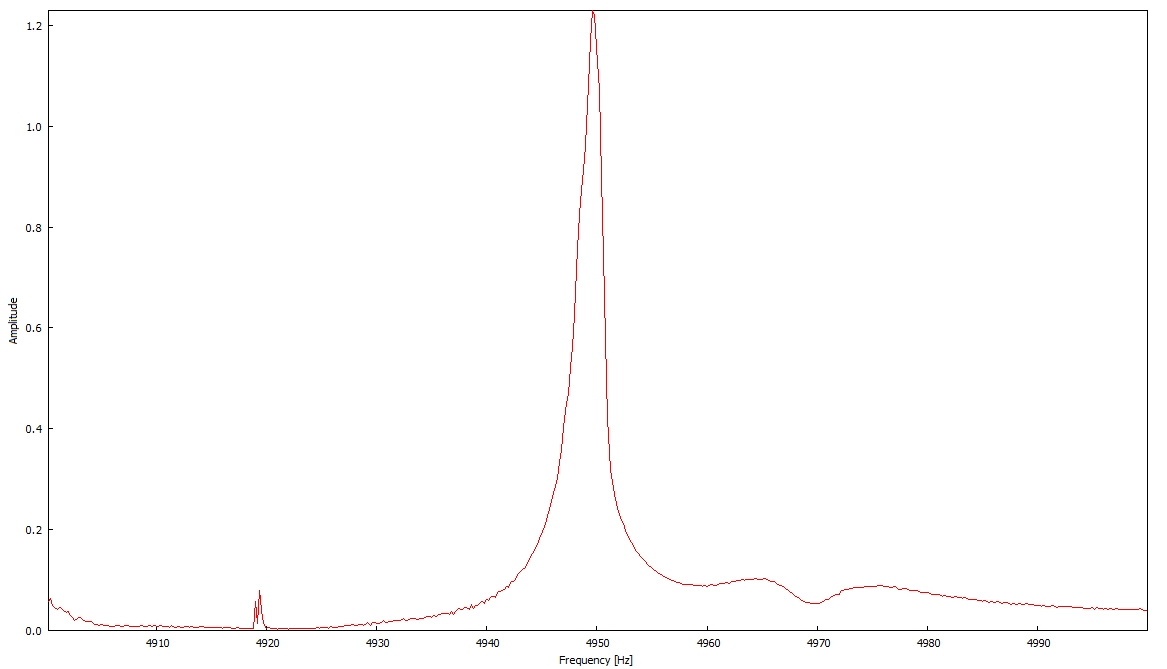
\includegraphics[width=\textwidth]{content/messungen/Chapter2new/2_2_0img.jpg}
\caption{Die dritte Resonanzstelle des Kugelresonators wird für $\alpha=0\degree$ zwischen 4.9~kHz und 5.0~kHz untersucht.}
\label{fig:2_2_0}
\end{figure}
\begin{figure}
\centering
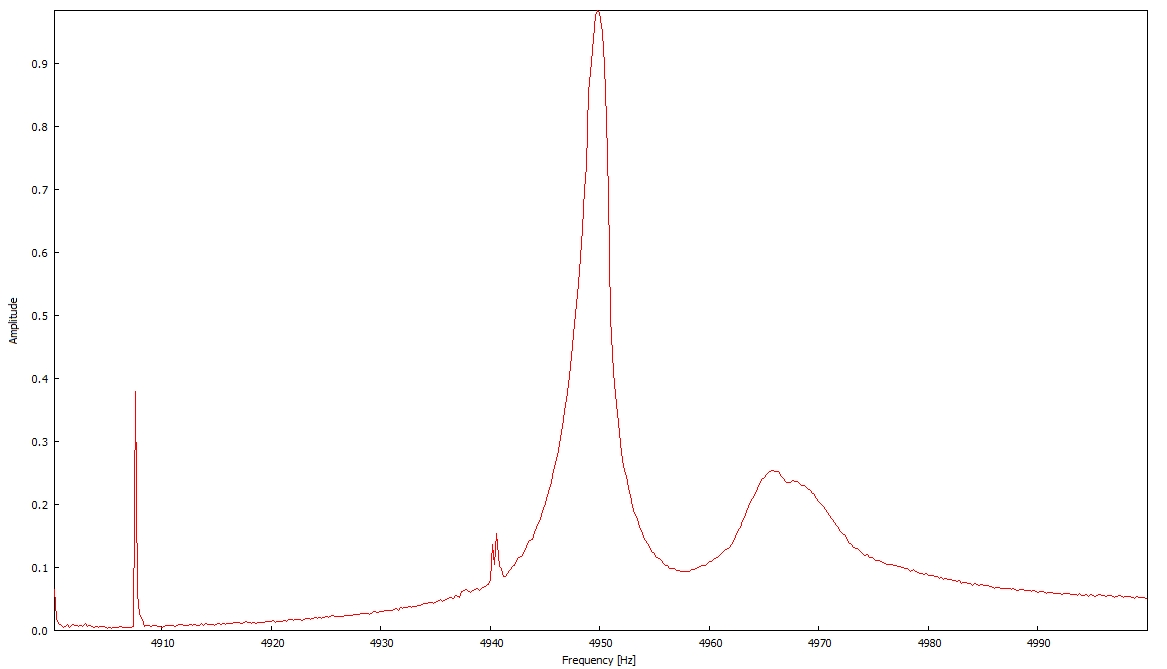
\includegraphics[width=\textwidth]{content/messungen/Chapter2new/2_2_20mg.jpg}
\caption{Die dritte Resonanzstelle des Kugelresonators wird für $\alpha=20\degree$ zwischen 4.9~kHz und 5.0~kHz untersucht.}
\label{fig:2_2_20}
\end{figure}
\begin{figure}
\centering
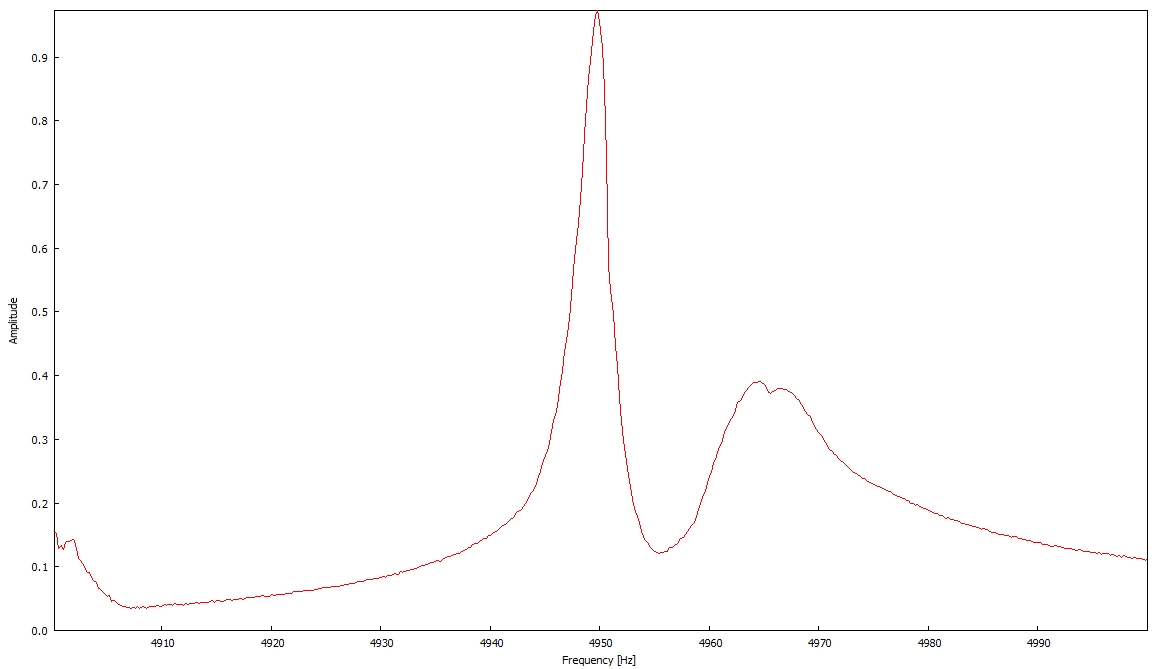
\includegraphics[width=\textwidth]{content/messungen/Chapter2new/2_2_40mg.jpg}
\caption{Die dritte Resonanzstelle des Kugelresonators wird für $\alpha=40\degree$ zwischen 4.9~kHz und 5.0~kHz untersucht.}
\label{fig:2_2_40}
\end{figure}
Um nun die Messungen an festen Resonanzstellen darzustellen wird das in Abbildung \ref{fig:2_3_180} aufgeführte von 2~kHz bis 7~kHz aufgenommene Spektrum betrachtet.
\begin{figure}
\centering
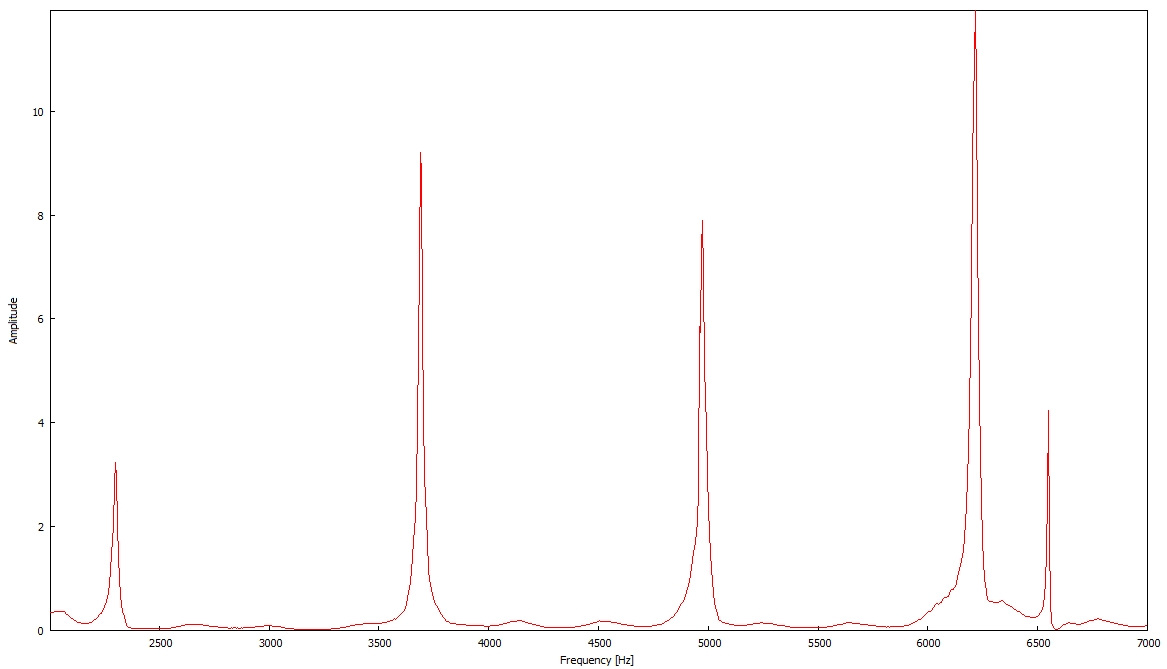
\includegraphics[width=\textwidth]{content/messungen/Chapter2new/2_3_180mg.jpg}
\caption{Spektrum des Kugelresonators von 2~kHz bis 7~kHz bei $\alpha=180\degree$.}
\label{fig:2_3_180}
\end{figure}
Die fünf zu erkennenden Resonanzstellen werden bei fester Frequenz durch variieren des Winkels $\alpha$ ausgemessen.
Es sei darauf hingewiesen, dass der Computer $\alpha$ automatisch in die gesuchte Größte $\theta$ umrechnet.
Um der Symmetrie des Kugelresonators gerecht zu werden, werden die Ergebnisse in den Polarplots \ref{fig:2_3_1} bis \ref{fig:2_3_5} dargestellt.
%%%%%%%%%%%%%%%%%%%%
\begin{figure}
\centering
\begin{subfigure}{0.4\textwidth}
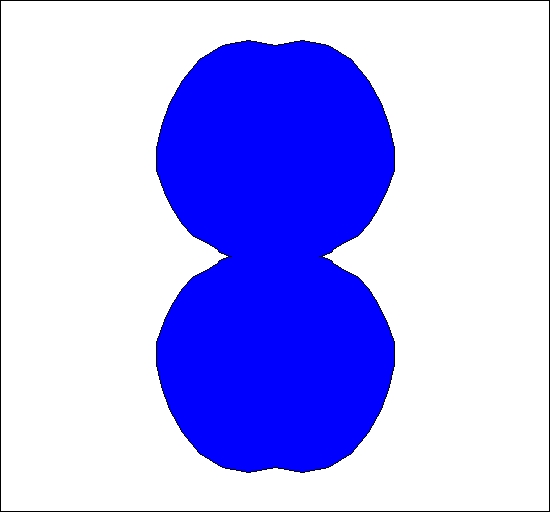
\includegraphics[width=\textwidth]{content/messungen/Chapter2new/2_3_1.jpg}
\subcaption{Frequenz ca. 2.30~kHz.}
\label{fig:2_3_1}
\end{subfigure}
\begin{subfigure}{0.4\textwidth}
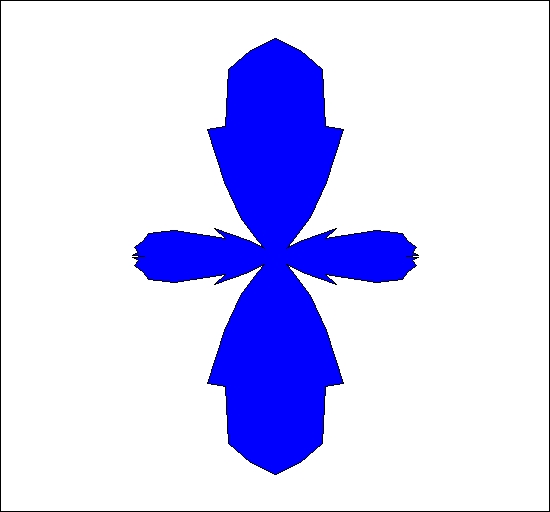
\includegraphics[width=\textwidth]{content/messungen/Chapter2new/2_3_2.jpg}
\subcaption{Frequenz ca. 3.69~kHz.}
\label{fig:2_3_2}
\end{subfigure}

\begin{subfigure}{0.4\textwidth}
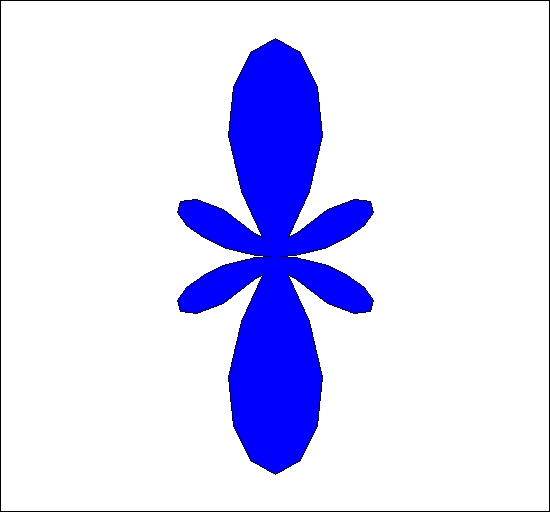
\includegraphics[width=\textwidth]{content/messungen/Chapter2new/2_3_3.jpg}
\subcaption{Frequenz ca. 4.98~kHz.}
\label{fig:2_3_3}
\end{subfigure}
\begin{subfigure}{0.4\textwidth}
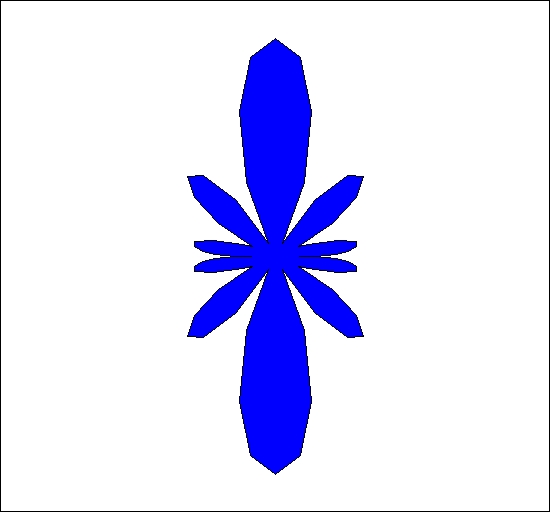
\includegraphics[width=\textwidth]{content/messungen/Chapter2new/2_3_4.jpg}
\subcaption{Frequenz ca. 6.21~kHze.}
\label{fig:2_3_4}
\end{subfigure}

\begin{subfigure}{0.4\textwidth}
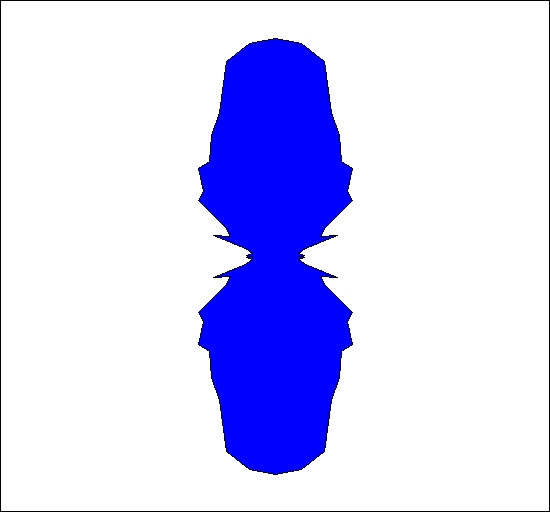
\includegraphics[width=\textwidth]{content/messungen/Chapter2new/2_3_5.jpg}
\subcaption{Frequenz ca. 6.55~kHz.}
\label{fig:2_3_5}
\end{subfigure}
\caption{Schallamplitude im Kugelresonator in Abhängigkeit des Winkels $\theta$.}
\end{figure}
%%%%%%%%%%%%%%%%%%%%%
\FloatBarrier
\subsection{Modell eines eindimensionalen Festkörpers}
\label{subsec:Modell eines eindimensionalen Festkörpers}
Die im Bereich zwischen 5~kHz und 9~kHz aufgenommenen Spektren der verschieden langen Röhren sind in den Abbildungen \ref{fig:4_1_75} bis \ref{fig:4_1_600} dargestellt.
Die Messung zeigt eine höhere Dichte der Resonanzen bei zunehmender Rohrlänge.
\begin{figure}
\centering
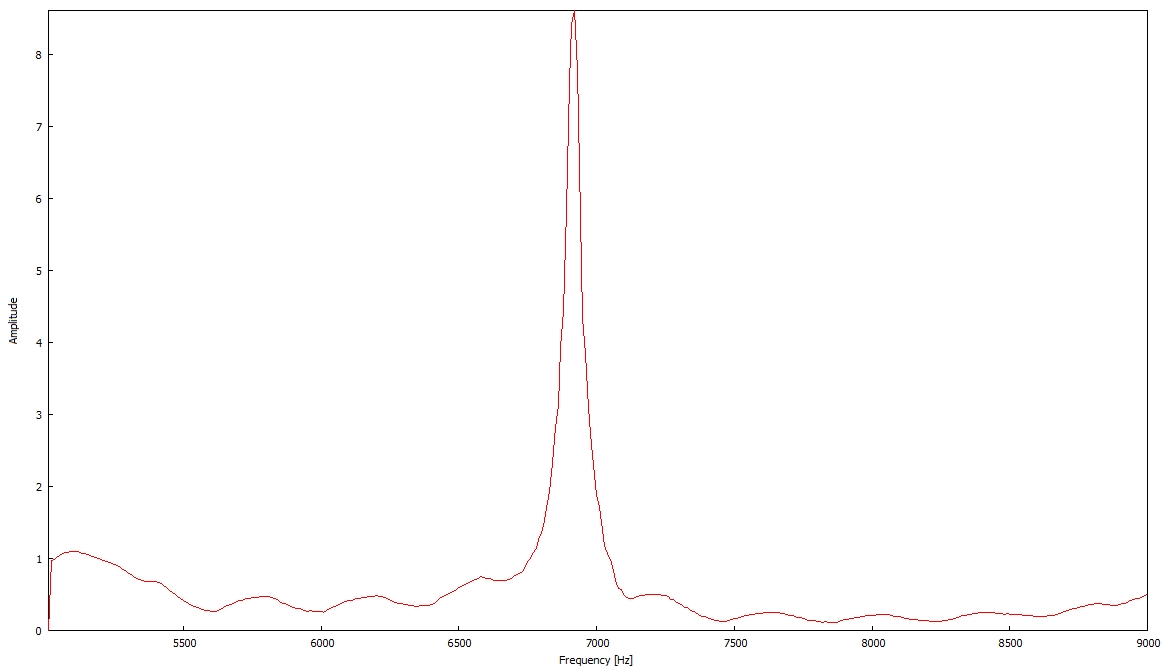
\includegraphics[width=1\textwidth]{content/messungen/Chapter4/4_1_75mm.jpg}
\caption{Spektrum einer 75~mm langen Röhre zwischen 5~kHz und 9~kHz.}
\label{fig:4_1_75}
\end{figure}

\begin{figure}
\centering
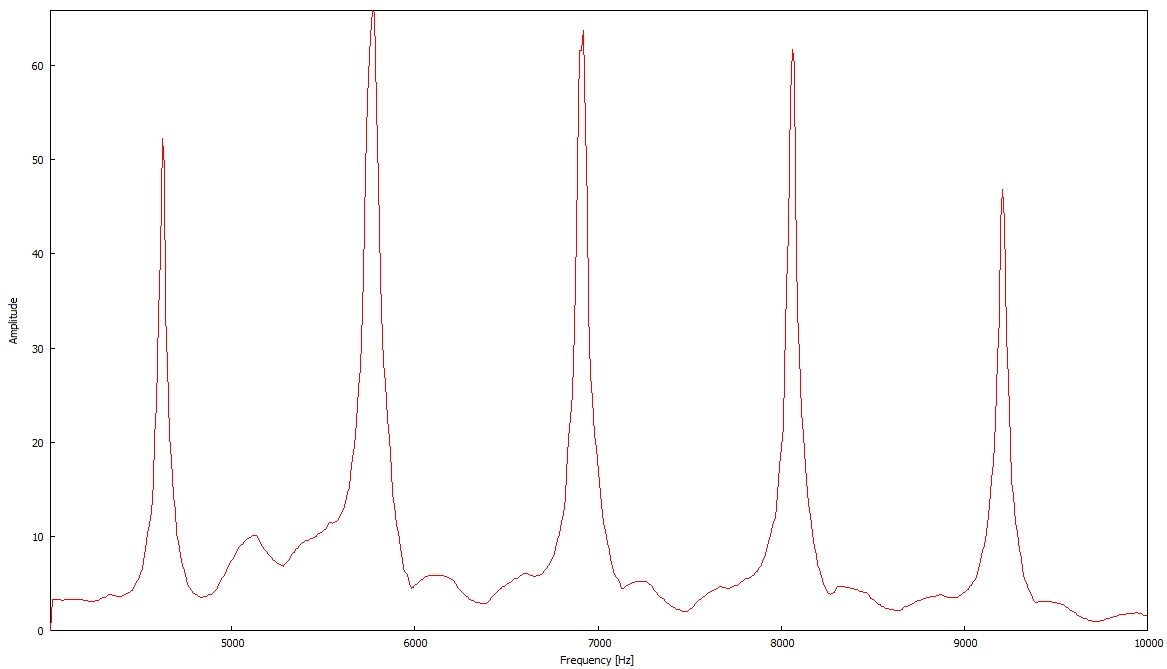
\includegraphics[width=1\textwidth]{content/messungen/Chapter4/4_1_150mm.jpg}
\caption{Spektrum einer 150~mm langen Röhre zwischen 4~kHz und 10~kHz.}
\label{fig:4_1_150}
\end{figure}

\begin{figure}
\centering
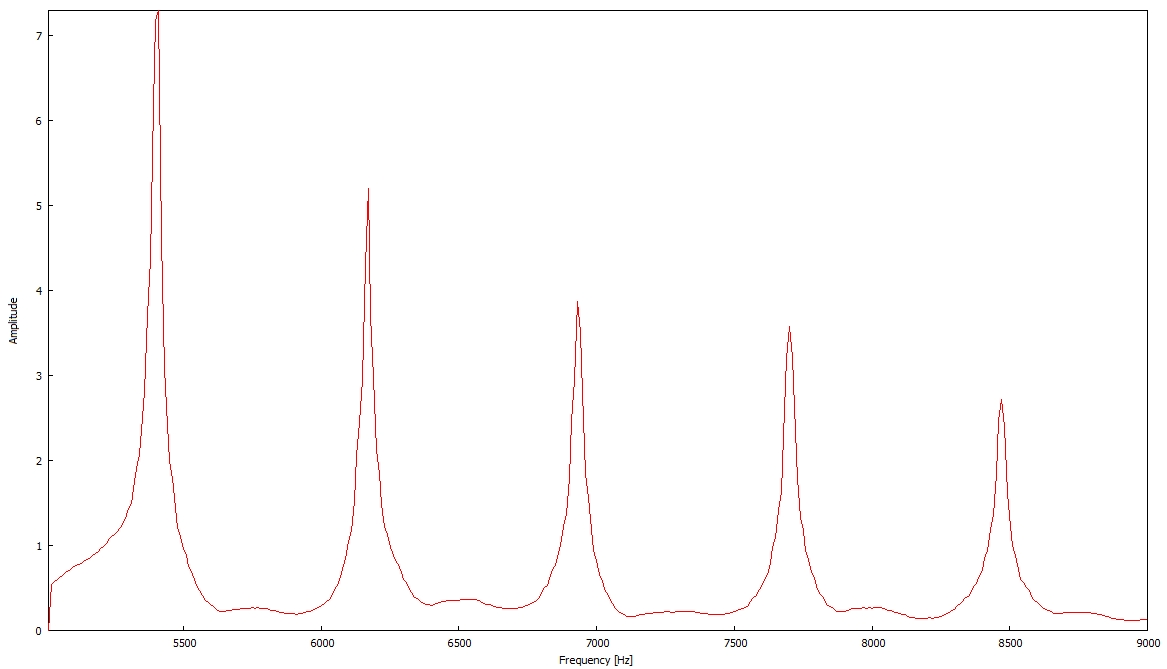
\includegraphics[width=1\textwidth]{content/messungen/Chapter4/4_1_225mm.jpg}
\caption{Spektrum einer 225~mm langen Röhre zwischen 5~kHz und 9~kHz.}
\label{fig:4_1_225}
\end{figure}

\begin{figure}
\centering
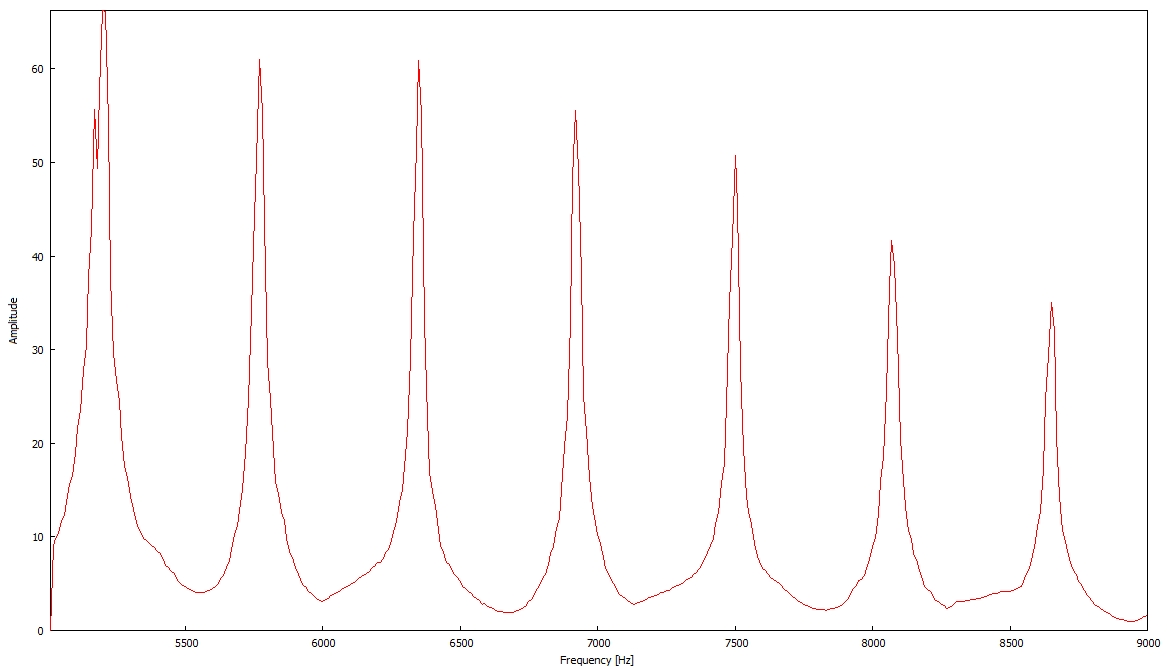
\includegraphics[width=1\textwidth]{content/messungen/Chapter4/4_1_300mm.jpg}
\caption{Spektrum einer 300~mm langen Röhre zwischen 5~kHz und 9~kHz.}
\label{fig:4_1_300}
\end{figure}

\begin{figure}
\centering
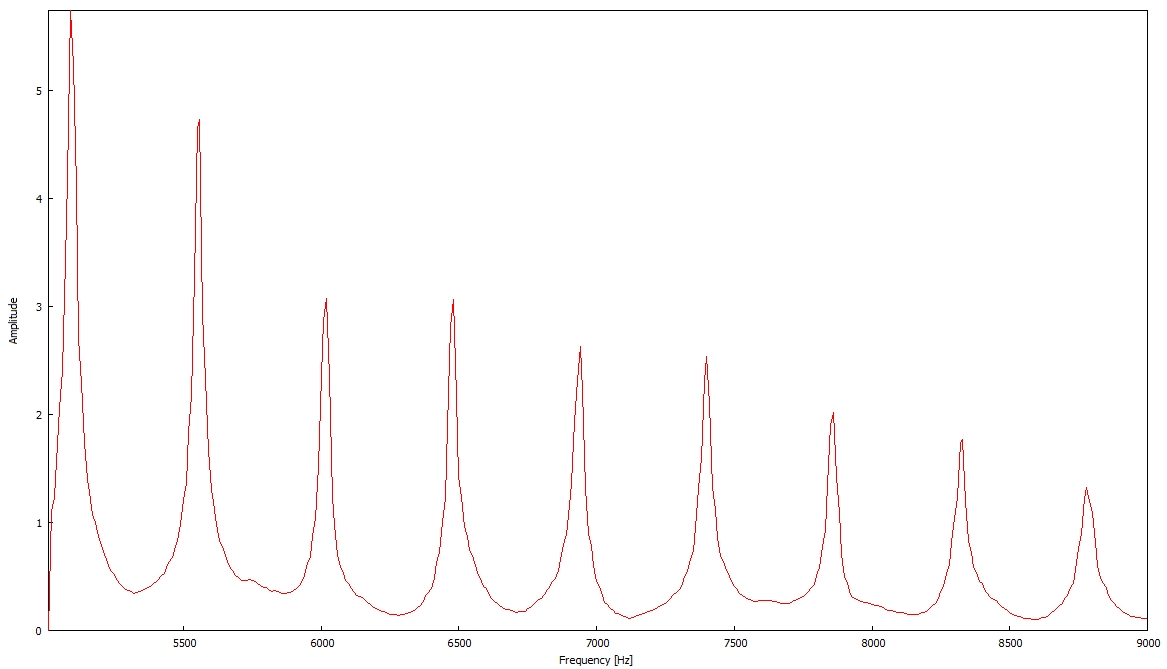
\includegraphics[width=1\textwidth]{content/messungen/Chapter4/4_1_375mm.jpg}
\caption{Spektrum einer 375~mm langen Röhre zwischen 5~kHz und 9~kHz.}
\label{fig:4_1_375}
\end{figure}

\begin{figure}
\centering
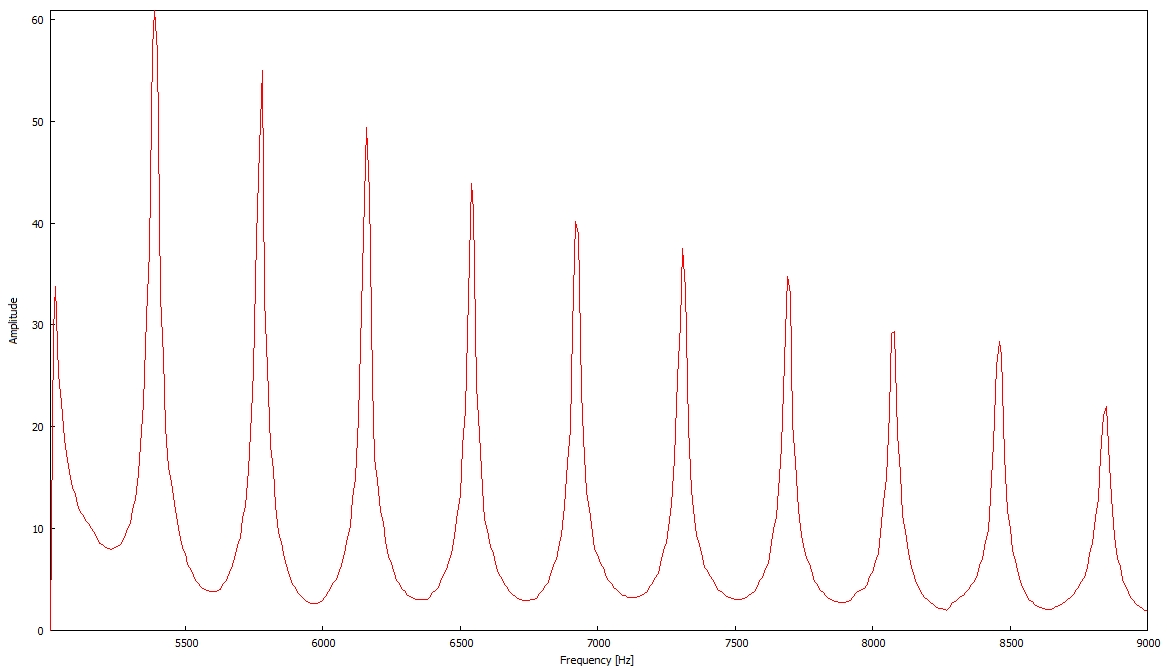
\includegraphics[width=1\textwidth]{content/messungen/Chapter4/4_1_450mm.jpg}
\caption{Spektrum einer 450~mm langen Röhre zwischen 5~kHz und 9~kHz.}
\label{fig:4_1_450}
\end{figure}

\begin{figure}
\centering
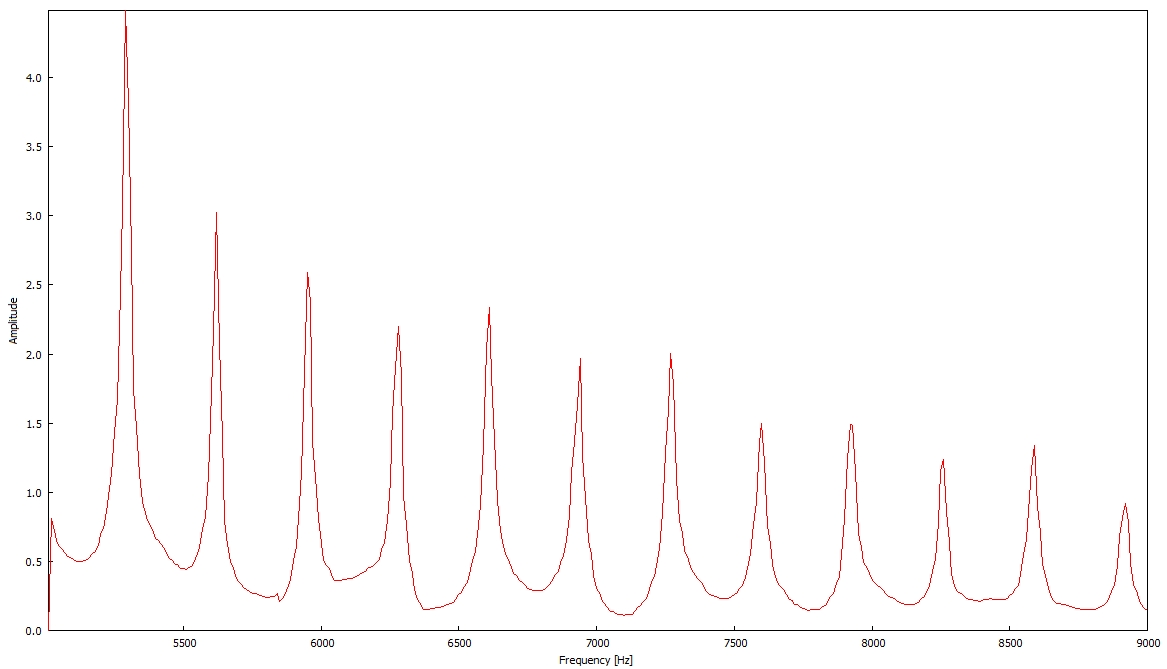
\includegraphics[width=1\textwidth]{content/messungen/Chapter4/4_1_525.jpg}
\caption{Spektrum einer 525~mm langen Röhre zwischen 5~kHz und 9~kHz.}
\label{fig:4_1_525}
\end{figure}

\begin{figure}
\centering
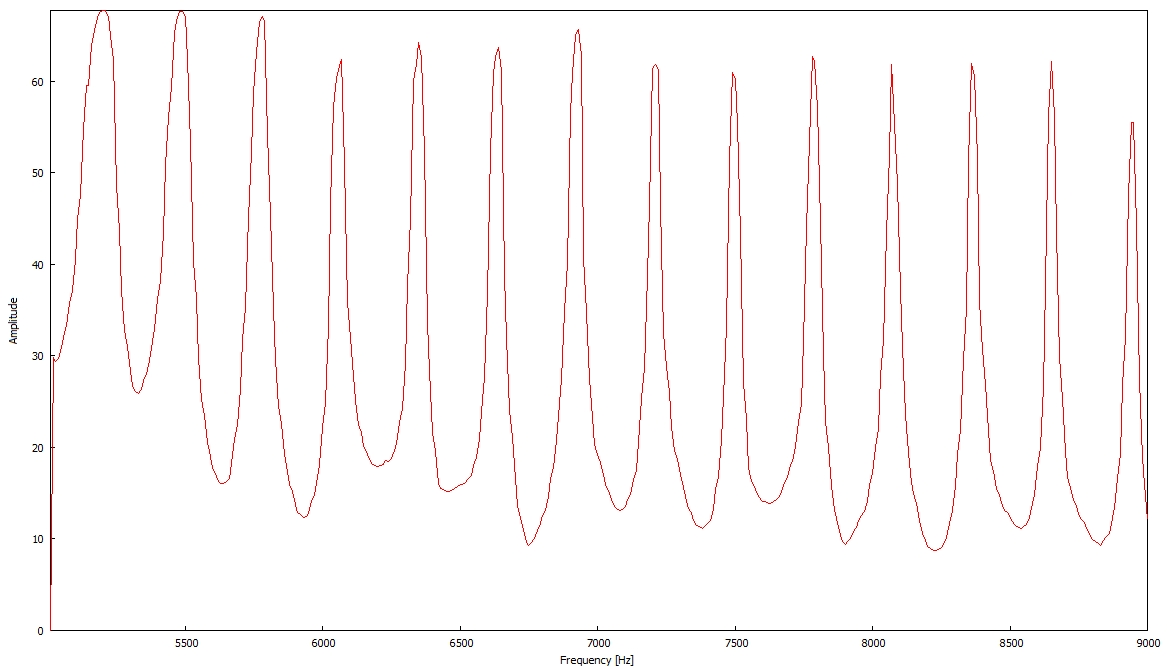
\includegraphics[width=1\textwidth]{content/messungen/Chapter4/4_1_600mm.jpg}
\caption{Spektrum einer 600~mm langen Röhre zwischen 5~kHz und 9~kHz.}
\label{fig:4_1_600}
\end{figure}
Die Peaks der Amplituden werden aus den Messdaten ausgelesen und werden in Tabelle \ref{tab:4:1} aufgeführt.
\begin{table}
\centering
\caption{Resonanzfrequenzen der verschiedenen Rohre im Frequenzbereich zwischen 5~kHz und 9~kHz, bzw. zwischen 4~kHz und 10~kHz für das Rohr der Länge 150~mm.}
\label{tab:4:1}
\begin{tabular}{c c c c c c c c c}
\hline
Rohrlänge  &600~mm&525~mm&450~mm&375~mm&300~mm& 225~mm& 150~mm & 75~mm \\ \hline
Resonanz- &5200& 5290& 5030 &5090 &5170 &5410 &4620 &6920\\
frequenzen&5480& 5620& 5390& 5560& 5770& 6170& 5770&\\
in Hz&5780& 5950& 5780& 6020& 6350& 6930& 6920&\\
&6070& 6280& 6160& 6480& 6920& 7700& 8060&\\
&6350& 6610& 6540& 6940& 7500& 8470& 9210&\\
&6640& 6940& 6920& 7400& 8070&& &\\
&6930& 7270& 7310& 7860& 8650&&&\\
&7210& 7600& 7690& 8330& &&&\\
&7490& 7920& 8080& 8780&&&&\\
&7780& 8260& 8460&&&&&\\
&8070& 8590&&&&&&\\
&8360& &&&&&&\\
&8650&&&&&&&\\
&8940&&&&&&&\\
\hline
\end{tabular}
\end{table}
Aus ihnen werden die Frequenzdifferenzen $\Delta f$ berechnet, um die Schallgeschwindigkeit zu bestimmen.
\begin{table}
\centering
\caption{Differenzen der Resonanzfrequenzen der verschiedenen Rohre im Frequenzbereich zwischen 5~kHz und 9~kHz, bzw. zwischen 4~kHz und 10~kHz für das Rohr der Länge 150~mm.}
\label{tab:4:2}
\begin{tabular}{c c c c c c c c c}
\hline
Rohrlänge  &600~mm&525~mm&450~mm&375~mm&300~mm& 225~mm& 150~mm & 75~mm \\ \hline
Differenz &280&330&360&470&600&760&1150&\\ 
der&300&330&390&460&580&760&1150&  \\ 
Resonanz-&290&330&380&460&570&770&1140&  \\ 
frequenzen&280&330&380&460&580&770&1150&  \\ 
in Hz&290&330&380&460&570&&&  \\ 
&290&330&390&460&580&  &  &  \\ 
&280&330&380&470&&  & &  \\ 
&280&320&390&450&  &  &  &  \\ 
&290&340&380&&  &  &  & \\ 
&290&330&&  &  &  &  &  \\ 
&290&&  &  &  &  &  &  \\ 
&290&  &  &  &  &  &  &  \\ 
&290&  &  &  &  &  &  & \\ 
\hline
Mittelwert&$287\pm 6$&$330\pm 4$&$381\pm 9$&$461\pm 6$&$580\pm 10$&$765\pm 5$&$1150\pm 4$ \\
in Hz &&&&&&&&\\
\hline
\end{tabular}
\end{table}
Mit 
\begin{align}
\Delta f=f_n-f_{n-1}=\frac{c}{\lambda_n}-\frac{c}{\lambda_{n-1}}=\frac{c}{2L}
\label{a:eq:1}
\end{align}
kann so aus den Mittelwerten der Frequenzdifferenzen aus Tabelle \ref{tab:4:2} die Schallgeschwindigkeit berechnet werden.
Es folgen die in Tabelle \ref{tab:4:3} aufgeführten Schallgeschwindigkeiten, deren Mittelwert 
\begin{align*}
c=(345\pm 2)~\text{ms}^{-1}
\end{align*}
das Ergebnis dieser Messung ist. Dabei wurde die Abweichung durch die Gauß'sche Fehlerfortpflanzung
\begin{align*}
\Delta c=\sqrt{\sum_{i=1}^n (\Delta c_i)^2}
\end{align*}
berechnet, wobei die $c_i$ die pro Rohr gemessenen Schallgeschwindigkeiten aus Tabelle \ref{tab:4:3} bezeichnen.
\begin{table}
\centering
\caption{Schallgeschwindigkeiten, berechnet nach Tabelle \ref{tab:4:2} und Gleichung (\ref{a:eq:1}).}
\label{tab:4:3}
\begin{tabular}{c c c c c c c c}
\hline
Rohrlänge in mm &600~mm&525~mm&450~mm&375~mm&300~mm& 225~mm& 150~mm \\ \hline
Schallgeschwindigkeit &$345\pm 7$&$347\pm 5$&$343\pm 8$&$346\pm 4$&$348\pm 6$&$344\pm 2$&$344\pm 1$\\
in ms$^{-1}$&&&&&&&\\
\hline
\end{tabular}
\end{table}
\FloatBarrier
Abbildung \ref{fig:4_2_1} zeigt ein Übersichtsspektrum eines 600~mm langen Rohres.
\begin{figure}
\centering
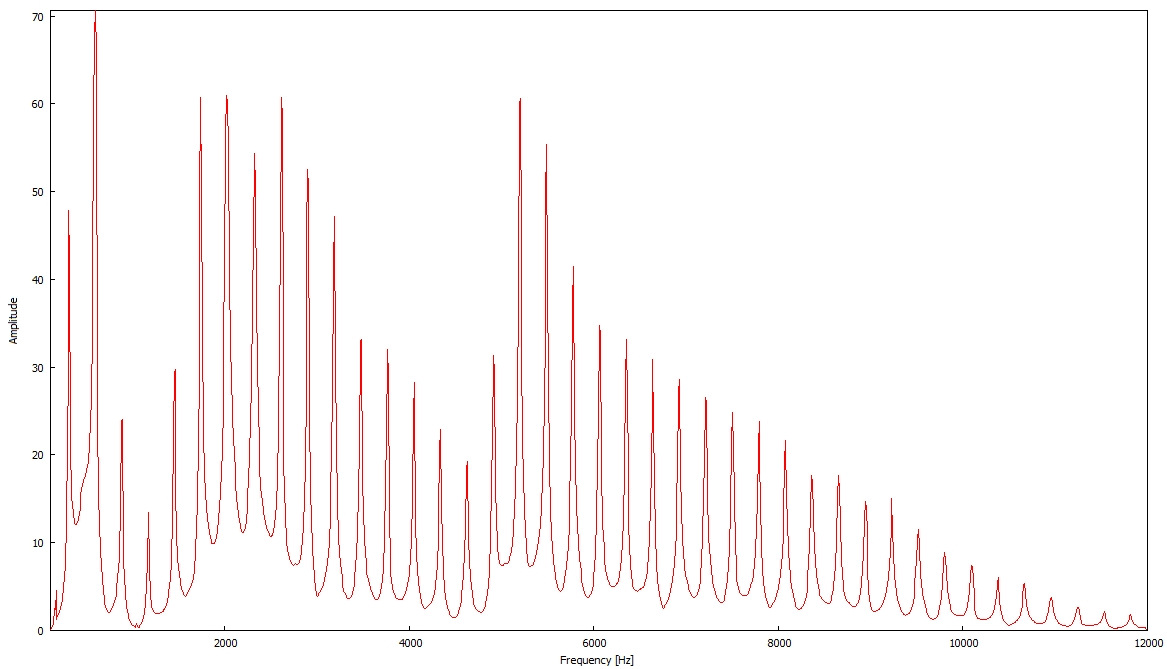
\includegraphics[width=1\textwidth]{content/messungen/Chapter4/4_2.jpg}
\caption{Resonanzspektrum eines Rohres der Länge 600~mm zwischen 0.1~kHz und 12~kHz.}
\label{fig:4_2_1}
\end{figure}
Durch abzählen der Peaks wird jedem Peak seine Wellenzahl
\begin{align}
k= n\frac{\pi}{L}
\end{align}
zugeordnet.
Abbildung \ref{fig:4_2_2} zeigt einen Plot der Resonanzfrequenzen gegen die entsprechenden Wellenzahlen.
\begin{figure}
\centering
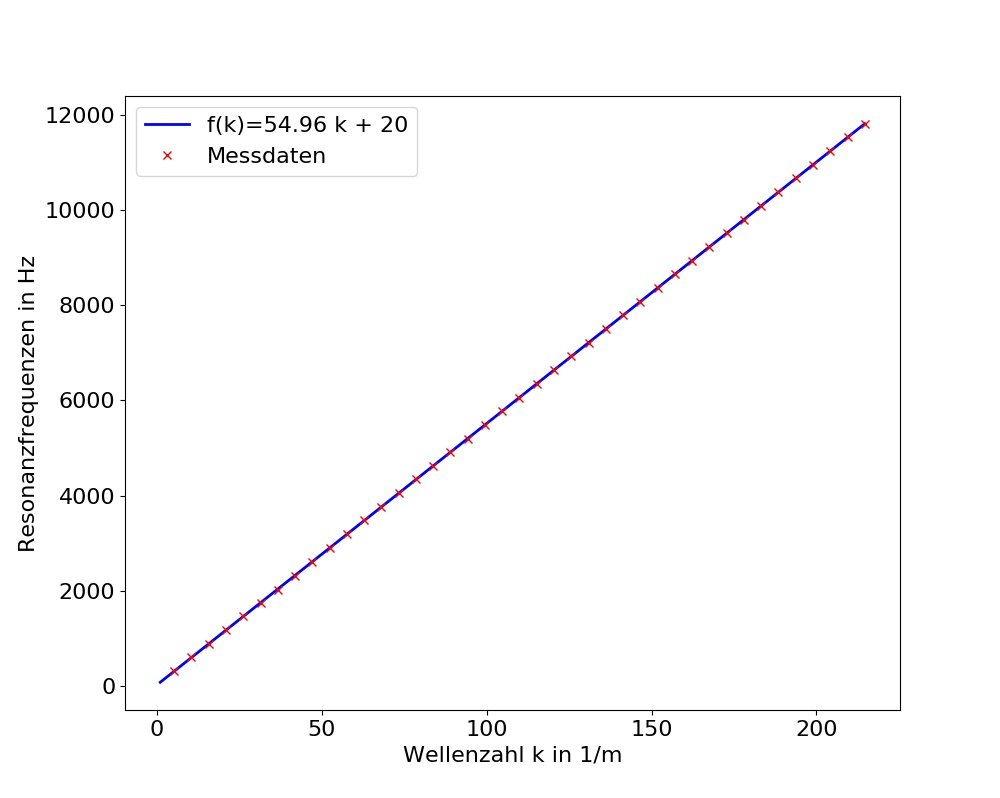
\includegraphics[width=\textwidth]{content/messungen/Chapter4/plot_4_2.jpg}
\caption{Resonanzfrequenzen in einem 600~mm Rohr in Abhängigkeit der Wellenzahl.}
\label{fig:4_2_2}
\end{figure}
Eine lineare Regression liefert die Ausgleichsgerade
\begin{align*}
f(k)=ak+b &&a=(54.96\pm 0.01)\text{ms}^{-1}&&b=(20\pm 1)\text{Hz} \text{ .}
\end{align*}
Es ist eindeutig eine lineare Dispersionsrelation zu erkennen.
Mit der bekannten Gleichung
\begin{align*}
f(k)=\frac{c}{2\pi}k
\end{align*}
lässt sich wiederholt die Lichtgeschwindigkeit 
\begin{align*}
c=(345.33\pm0.06)\text{ms}^{-1}
\end{align*}
berechnen.
\FloatBarrier
Nun wird das 400~mm lange Rohr bestehend aus 8 Einheiten der Länge 50~mm und 6 Blenden mit den Durchmessern $d=10,13,16~mm$ betrachtet.
Die Abbildungen \ref{fig:4_3_10} bis \ref{fig:4_3_16} zeigen die zugehörigen Resonanzspektren.
Für alle drei Blendendurchmesser stimmen die Wellenzahlen der Bänder überein.
Das erste Band liegen zwischen den Wellenzahlen $k^1_\text{min}=5.24~\text{m}^{-1}$ und $k^1_\text{max}=31.42~\text{m}^{-1}$, das zweite zwischen $k^2_\text{min}=36.65~\text{m}^{-1}$ und $k^2_\text{max}=62.83~\text{m}^{-1}$ und das dritte zwischen $k^3_\text{min}=68.07~\text{m}^{-1}$ und $k^3_\text{max}=94.25~\text{m}^{-1}$.
Resonanzstellen des vierten Bandes sind nicht alle klar erkennbar. 
Die Wellenzahlen dieses Bandes liegen zwischen $k^4_\text{min}=99.48~\text{m}^{-1}$ und $k^4_\text{max}=125.57~\text{m}^{-1}$.
Zwischen den Bändern ist jeweils eine Bandlücke.

\begin{figure}
\centering
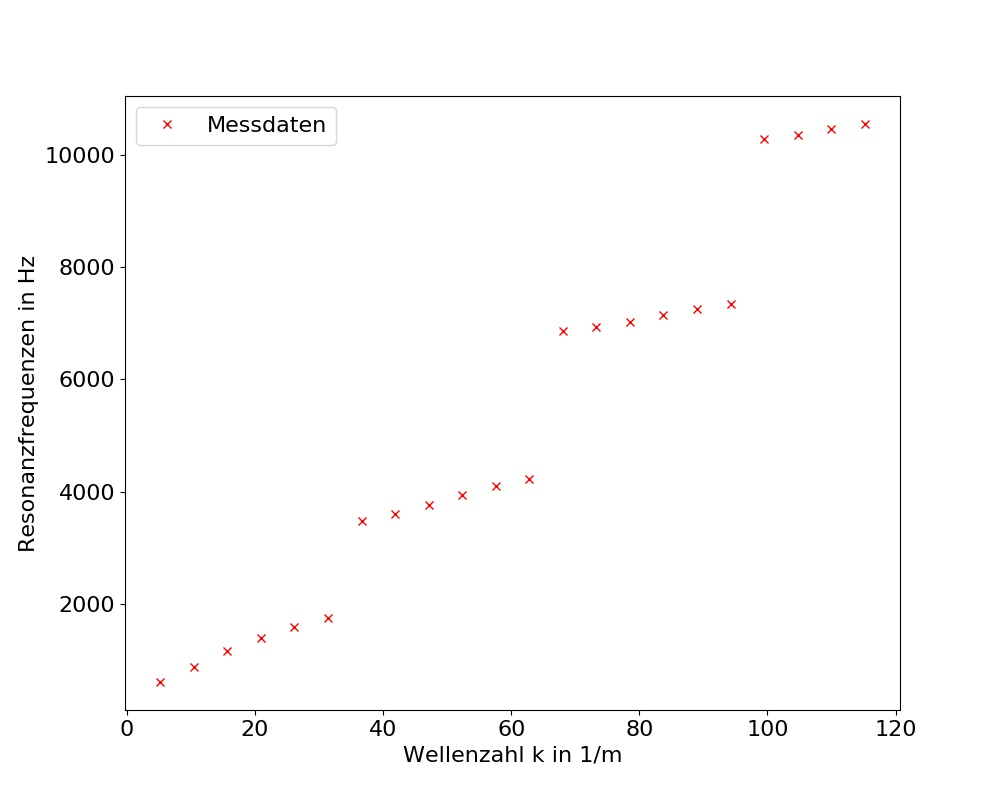
\includegraphics[width=\textwidth]{content/messungen/Chapter4/plot_4_3_10}
\caption{Resonanzspektrum eines 400~mm langen Rohres mit 6 10~mm Blenden, jeweils im Abstand von 50~mm, zwischen 0.1~kHz und 12~kHz.}
\label{fig:4_3_10}
\end{figure}
\begin{figure}
\centering
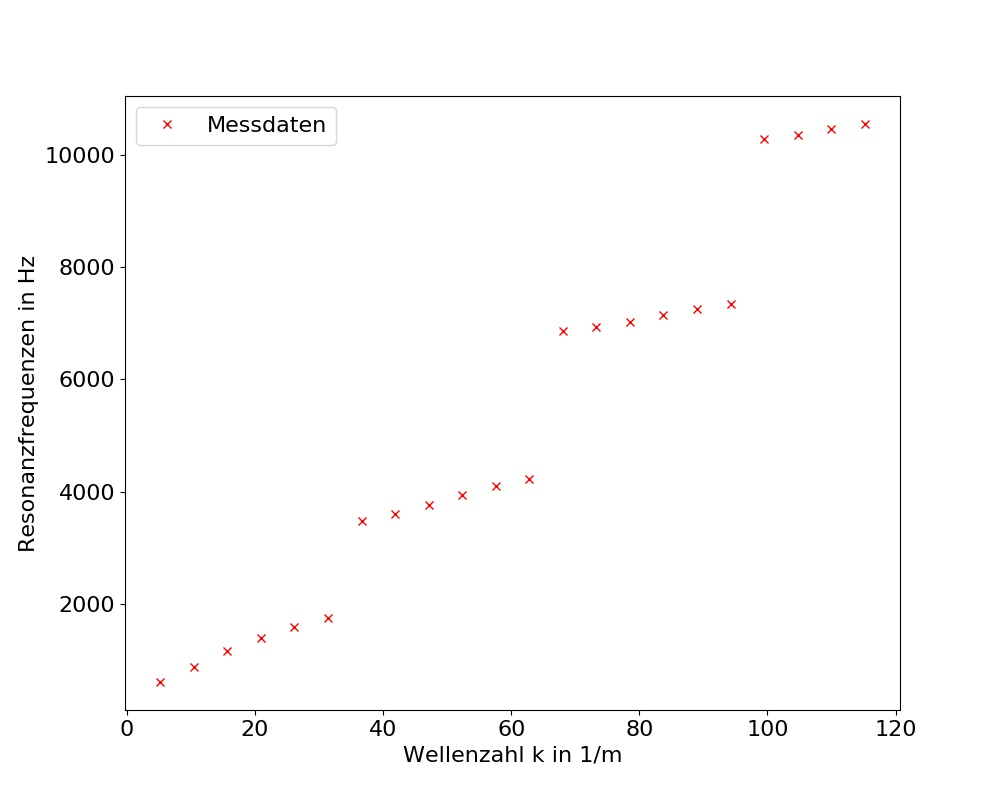
\includegraphics[width=\textwidth]{content/messungen/Chapter4/plot_4_3_13}
\caption{Resonanzspektrum eines 400~mm langen Rohres mit 6 13~mm Blenden, jeweils im Abstand von 50~mm, zwischen 0.1~kHz und 12~kHz.}
\label{fig:4_3_13}
\end{figure}
\begin{figure}
\centering
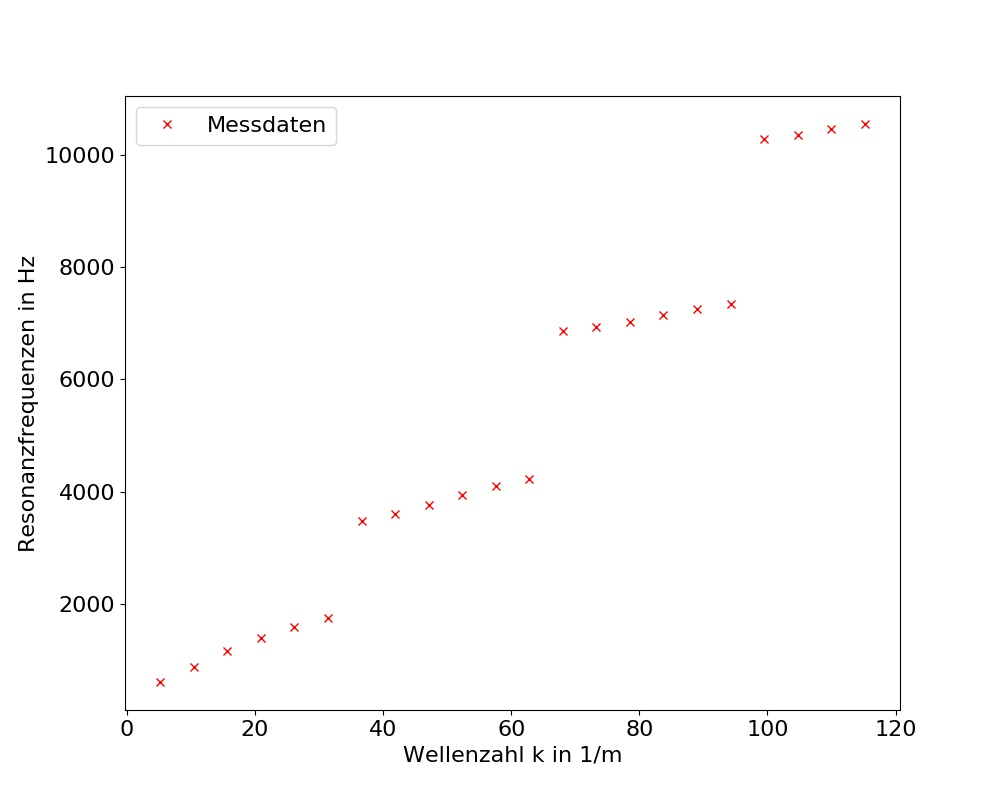
\includegraphics[width=\textwidth]{content/messungen/Chapter4/plot_4_3_16}
\caption{Resonanzspektrum eines 400~mm langen Rohres mit 6 16~mm Blenden, jeweils im Abstand von 50~mm, zwischen 0.1~kHz und 12~kHz.}
\label{fig:4_3_16}
\end{figure}
